\documentclass[border=3pt]{standalone}
% Preâmbulo compartilhado pelos diagramas TikZ da aula 7 de IHC (Organização do Espaço de Problema)
\usepackage[T1]{fontenc}
\usepackage[utf8]{inputenc}
\usepackage{lmodern}
\usepackage{amsmath}
\usepackage{xcolor}
\usepackage{tikz}
\usetikzlibrary{arrows.meta,angles,quotes,decorations.pathmorphing,calc,
                positioning,shapes.geometric,shapes.misc,backgrounds,fit,
                math}

% Paleta (mesma dos SVGs originais)
% Paleta da disciplina de IHC: acento roxo (#755099), da capa do livro.
% (o nome "dblue" é mantido para não alterar todos os diagramas)
\definecolor{dblue}{HTML}{755099}
\definecolor{dorange}{HTML}{B3541E}
\definecolor{dgreen}{HTML}{4A7C59}
\definecolor{dred}{HTML}{9C4B4B}
\definecolor{dcream}{HTML}{F4F1EA}
\definecolor{dshade}{HTML}{DDD7C9}

% Função gaussiana (não normalizada por padrão de escala visual)
\pgfmathdeclarefunction{gauss}{3}{%
  \pgfmathparse{1/(#3*sqrt(2*pi))*exp(-((#1-#2)^2)/(2*#3^2))}%
}

% Estilos comuns (prefixo d... para não colidir com chaves internas do pgf)
\tikzset{
  >={Stealth[length=2mm]},
  dguide/.style={gray!55, dashed, line width=0.4pt},
  daxis/.style={gray!60, line width=0.7pt, ->},
  dbody/.style={fill=black!3, draw=black!80, line width=1pt},
  dacc/.style={draw=dblue, line width=1pt},
  dlbl/.style={black!55, font=\small},
  dsub/.style={black!45, font=\footnotesize},
  dstate/.style={circle, draw=black!80, fill=dcream, line width=1pt,
                 minimum size=17mm, font=\large, inner sep=1pt},
  dobs/.style={circle, draw=black!80, fill=dshade, line width=1pt,
               minimum size=14mm, font=\large, inner sep=1pt},
  dbox/.style={rounded corners=2pt, draw=black!80, fill=dcream, line width=1pt,
               align=center, inner sep=6pt},
  dop/.style={circle, draw=black!80, fill=white, line width=1pt,
              minimum size=6mm, inner sep=0pt, font=\small},
  dtrans/.style={->, dblue, line width=1pt},
  dmeas/.style={->, dorange, line width=1pt},
  dcurve/.style={line width=1pt, dblue},
  dcurveb/.style={line width=1.4pt, dorange},
}

\begin{document}
\hyphenpenalty=10000 \exhyphenpenalty=10000 \tolerance=9999 \emergencystretch=3em
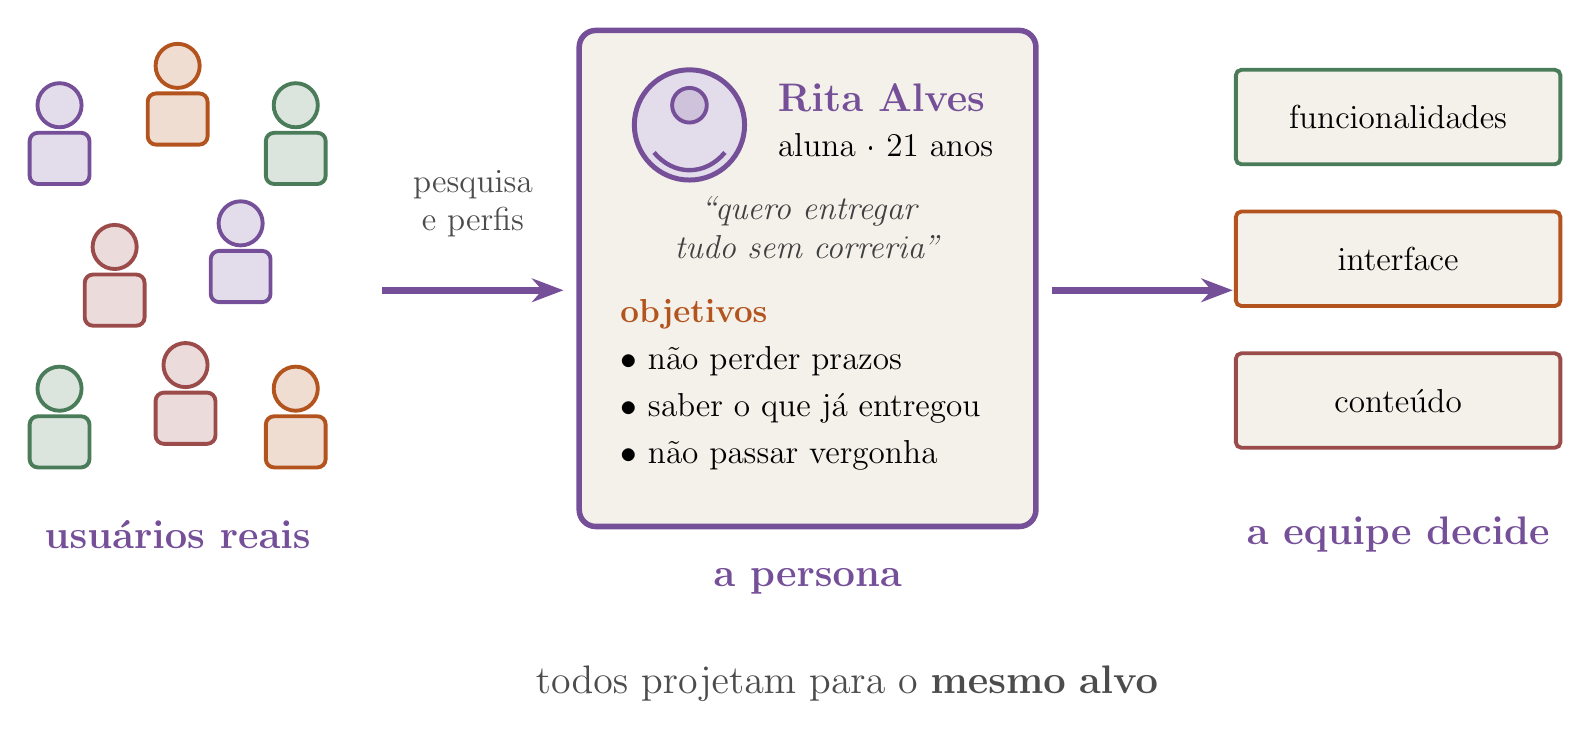
\begin{tikzpicture}[x=1cm,y=1cm]
  % usuarios reais: bonequinhos variados
  \foreach \x/\y/\c in {0.0/5.4/dblue, 1.5/5.9/dorange, 3.0/5.4/dgreen, 0.7/3.6/dred, 2.3/3.9/dblue, 0.0/1.8/dgreen, 1.6/2.1/dred, 3.0/1.8/dorange} {
    \draw[\c, fill=\c!20, line width=1.4pt] (\x,\y+0.55) circle (0.28);
    \draw[\c, fill=\c!20, line width=1.4pt, rounded corners=3pt] (\x-0.38,\y-0.45) rectangle (\x+0.38,\y+0.2);
  }
  \node[font=\Large\bfseries, dblue] at (1.5,0.5) {usuários reais};
  \draw[dtrans, line width=2.4pt, -{Stealth[length=4mm]}] (4.1,3.6) -- (6.4,3.6);
  \node[font=\large, black!70, text width=2.4cm, align=center] at (5.25,4.7) {pesquisa e perfis};
  % cartao de persona
  \draw[dblue, fill=dcream, line width=2pt, rounded corners=6pt] (6.6,0.6) rectangle (12.4,6.9);
  \draw[dblue, fill=dblue!20, line width=1.8pt] (8.0,5.7) circle (0.7);
  \draw[dblue, fill=dblue!35, line width=1.4pt] (8.0,5.95) circle (0.22);
  \draw[dblue, line width=1.6pt] (7.55,5.35) .. controls (7.8,5.05) and (8.2,5.05) .. (8.45,5.35);
  \node[font=\Large\bfseries, dblue, anchor=west] at (9.0,6.05) {Rita Alves};
  \node[font=\large, anchor=west] at (9.0,5.45) {aluna · 21 anos};
  \node[font=\large\itshape, black!75, text width=5.2cm, align=center] at (9.5,4.4) {``quero entregar tudo sem correria''};
  \node[font=\large\bfseries, dorange, anchor=west] at (7.0,3.3) {objetivos};
  \node[font=\large, anchor=west] at (7.0,2.7) {$\bullet$ não perder prazos};
  \node[font=\large, anchor=west] at (7.0,2.1) {$\bullet$ saber o que já entregou};
  \node[font=\large, anchor=west] at (7.0,1.5) {$\bullet$ não passar vergonha};
  \node[font=\Large\bfseries, dblue] at (9.5,-0.1) {a persona};
  \draw[dtrans, line width=2.4pt, -{Stealth[length=4mm]}] (12.6,3.6) -- (14.9,3.6);
  % equipe decide
  \tikzset{e/.style={dbox, text width=3.7cm, minimum height=1.2cm, font=\large, line width=1.4pt}}
  \node[e, draw=dgreen] at (17.0,5.8) {funcionalidades};
  \node[e, draw=dorange] at (17.0,4.0) {interface};
  \node[e, draw=dred] at (17.0,2.2) {conteúdo};
  \node[font=\Large\bfseries, dblue] at (17.0,0.5) {a equipe decide};
  \node[font=\Large, black!70, text width=9cm, align=center] at (10.0,-1.4) {todos projetam para o \textbf{mesmo alvo}};
\end{tikzpicture}
\end{document}
